The main goal of the Optimization System (OS) is to produce solutions to user defined FTP instances. Upon defining an itinerary and translating it to a FTP instance, the arcs which connect the nodes are not defined, and thus, no valid solution can be produced. Thus, the OS is heavily dependent on the Data Management system, as it requires relevant flight data to process the requests. 

Depending on the particular request being processed, the required time to collect all the necessary flights, or the time to run a computationally heavy optimization algorithm, might be very high. Because of this, the optimization system is distributed into different layers, as illustrated in figure \ref{fig:optimization_system}, which require different amounts of information regarding the flights, and produce multiple solutions using different heuristics, at different times. The goal of this is to reduce the latency that is sensed by the user, by producing an initial solution as soon as possible, and continue to search for a better one afterwards.

\begin{figure}[htpb]
  \centering
  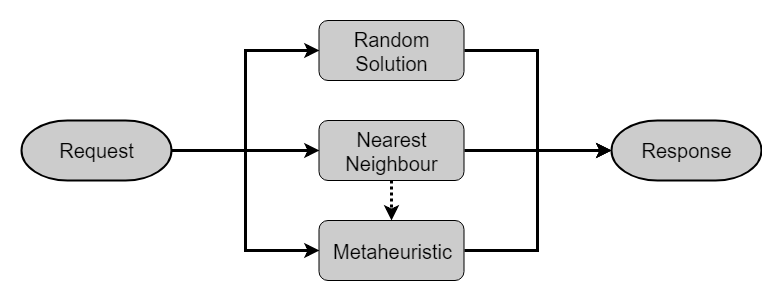
\includegraphics[width=\textwidth]{./Figures/system_design/utility.png}
  \caption{Simplified illustration of the optimization system, which utilizes different algorithms 
  to produce a solution to a user defined request.}
  \label{fig:optimization_system}  
\end{figure}

The first layer of the optimization system implements a random solution, as proposed in section \ref{sec:pseudo_random}. This procedure allows the construction of a solution in a very fast manner, as it randomly selects one node after another, and only requires information regarding a very limited number of flights. Despite producing a very fast solution, the quality of it is expected to be low.

The second layer of the OS implements the nearest neighbour heuristics proposed in section \ref{sec:nn}. The implementation of this heuristic requires information regarding the entire weight matrix associated to the problem. Because of this, it must run only after constructing the initial solution. It is expected that the solution constructed by this procedure is of higher quality to the initial one.

In its turn, the third layer of the OS implements the meta-heuristic optimization algorithms proposed in section \ref{sec:aco} and \ref{sec:sa}. Similarly to the nearest neighbour heuristic, these optimization algorithms require information regarding the entire weight matrix. Thus, they must also run only after the initial solution construction procedure, but they might run in parallel with the nearest neighbour heuristic. It is expected that the solutions constructed by these meta-heuristics are of much better quality than the initial and the nearest neighbour solutions.

\todo{Nota do professor: nao se percebe se os metodos correm sequencialmente ou em paralelo}

\todo{Eles na pratica correm sequencialmente. Isto e algo que devemos abordar aqui, ou so no proximo capitulo?}

